% % % % % % % % % % % % % % 
% 
% Skript zu NUMERIK I
% WS14/15
% von Prof. Dr. Blank
% Universität Regensburg
% 
% 
%	Kap. 2: Lineare Gleichungssysteme: Direkte Methoden
% 
% % % % % % % % % % % % % % 


\chapter{Lineare Gleichungssysteme: Direkte Methoden}
Sei $ A \in \R^{n\times n}$, $b \in \R^n$. Gesucht ist $x\in \R^n$ mit 
\begin{gather*}
  A\cdot x = b
\end{gather*}
Weitere Voraussetzungen sind die Existenz und Eindeutigkeit einer
Lösung.

Bemerkungen hierzu:
\begin{itemize}
\item Ein verlässlicher Lösungsalgorithmus überprüft dies und behandelt alle Fälle. 
\item Die Cramersche Regel ist ineffizient (s. Einführung
  \ref{CramerscheRegel}).
\item Das Inverse für $x=A^{-1}\cdot b$ aufzustellen ist ebenso ineffizient,
  denn es ist keine Lösung für alle $b\in \R^n$ verlangt
  und der Algorithmus wird evtl. instabil aufgrund vieler Operationen.
\item [$\Rightarrow$] Invertieren von Matrizen vermeiden!!
\item [$\Rightarrow$] Lösen des Linearen Gleichungssystems!!
\end{itemize}

\sectione{Gaußsches Eliminationsverfahren} \label{2.2.1}
\index{Gaußsches Eliminationsverfahren}\index{Dreieckszerlegung}
Das Verfahren wurde 1809 von Friedrich Gauß,
1759 von Josepf Louis Lagrange beschrieben
und war seit dem 1. Jhd. v. Chr. in China bekannt.

\subsectione{Vorwärtselimination} \label{2.1.1}
\index{Vorwärtselimination}\index{Vorwärtssubstitution}
Das Gaußverfahren gilt der Lösung eines linearen Gleichungssystems der Form
\begin{align*}
  Ax &= b
\end{align*}
mit $A=(a_{ij})_{i,j \leq n} \in K^{n\times n}$ Matrix und $b=(b_i)_{i\leq n} \in K^n$ Vektor.\\
Der zugehörige Algorithmus sieht folgendermaßen aus:
\begin{gather*}
  \begin{array}{ccccccccc}
    a_{11}x_1 &+& a_{12}x_2 &+& \cdots &+& a_{1n}x_n & = & b_1 ~~\\
    a_{21}x_1 &+& a_{22}x_2 &+& \cdots &+& a_{2n}x_n & = & b_2 \\
    \vdots         &&        \vdots     &&              &&   \vdots       &    & \vdots \\
    a_{n1}x_1 &+& a_{n2}x_2 &+& \cdots &+& a_{nn}x_n & = & b_n \\\\
              &&&& \Downarrow &&&& 
  \end{array} \\
  \quad	(\text{$i$-te Zeile}) - (\text{1. Zeile})\cdot \frac{a_{i1}}{a_{11}} \Rightarrow a_{i1}=0\\
  \begin{array}{ccccccccc}
    &&&& \Downarrow &&&&  \\\\
    a_{11}x_1 &+& a_{12}x_2 &+& \cdots &+& a_{1n}x_n & = & b_1 \\
    &+& a_{22}^{(1)}x_2 &+& \cdots &+& a_{2n}^{(1)}x_n & = & b_2^{(1)} \\
    &&        \vdots     &&              &&   \vdots       &    & \vdots \\
    && && && a_{nn}^{(1)}x_n & = & b_n^{(1)} \\\\
    &&&& \Downarrow &&&&\\
    &&&& \vdots &&&&
  \end{array} 
\end{gather*}
mit
\begin{align*}
  a_{ij}^{(1)} &= a_{ij}-a_{1j}\cdot \frac{a_{i1}}{a_{11}}
  & \text{für }i,j = 2, \cdots, n \\
  b_i^{(1)}      &= b_i- b_1\cdot \frac{a_{i1}}{a_{11}}
  & \text{für }i = 2, \cdots, n 
\end{align*}

% --------------------------------------------------------

In jedem Schritt werden die Einträge der $k$-ten Spalte analog 
unterhalb der Diagonalen (also $k=1, \cdots, n-1$) eliminiert:
\marginpar{08.10.2014}
\begin{align*}
  (\text{$i$-te Zeile})- (\text{$k$-te Zeile})\cdot\frac{a_{ik}}{a_{kk}}
  && \text{für } i=k+1, \cdots ,n 
\end{align*}
Die Reihe 
\begin{gather*}
  A \rightarrow A^{(1)} \rightarrow A^{(2)} \rightarrow \dotsm \rightarrow A^{(n-1)}
\end{gather*}
wird bis zum $n$-ten Schritt fortgeführt, d.h. bis eine obere Dreiecksgestalt eintritt:
\begin{align}
  \nonumber
  \underbrace{	\begin{pmatrix}
      a_{11} & \dotsm & \dotsm & a_{1n} \\
      & a_{22}^{(1)} & \dotsm & a_{2n}^{(1)} \\
      &&              \ddots  &  \vdots \\
      0        && &                             a_{nn}^{(n-1)}
    \end{pmatrix}}_{\coloneqq R}
                    \cdot
                    \begin{pmatrix}
                      x_1 \\
                      x_2 \\
                      \vdots \\
                      x_n
                    \end{pmatrix}
             & =
               \underbrace{\begin{pmatrix}
                   b_1 \\
                   b_2^{(1)} \\
                   \vdots \\
                   b_n^{(n-1)}
                 \end{pmatrix}}_{\coloneqq z} \\
  Rx &= z 	\label{II.1.1} 
\end{align}
wobei für  $i=k+1, \cdots ,n$ die Einträge wie folgt aussehen:
\begin{align}	
  l_{ik} &\coloneqq \frac{a_{ik}^{(k-1)}}{a_{kk}^{(k-1)}} \label{II.1.2} \\
  a_{ij}^{(k)} &= a_{ij}^{(k-1)} - a_{kj}^{(k-1)}\cdot l_{ik} \label{II.1.3}
               & \text{für } j=k+1, \cdots , n\\ %
  b_i^{(k)} &= b_i^{(k-1)} -b_k^{(k-1)} \cdot   l_{ik}
              \label{II.1.4}\index{Vorwärtssubstitution}
\end{align}
Dieser Prozess wird \textbf{Vorwärtselimination} genannt.\\

Der zugehörige Algorithmus ist:

\begin{pseudocode}{0.5\linewidth}
  \textbf{for} $ k = 1, \ldots , n-1$\\
  |~	\> \textbf{for} $i = k + 1, \ldots , n$ \\
  |~	\> |~\> $l_{ik} = a_{ik} /a_{kk}$\\
  |~	\> |~\> \textbf{for} $j = k + 1, \ldots , n$ \\
  |~	\> |~\>|~\> $a_{ij} = a_{ij} - l_{ik} a_{kj} $\\
  |~	\> |~\> \textbf{end}\\
  |~	\> |~\> $b_i = b_i -  l_{ik} b_k $\\
  |~	\> \textbf{end} \\
  \textbf{end}
\end{pseudocode}

\subsectione{Rückwärtselimination}\label{2.1.2}
Für die Lösung des Gleichungssystems ist dann noch die
\textbf{Rückwärtssubstitution} \index{Rückwärtssubstitution} nötig:
\begin{align}
  x_n &= \frac{b_n^{(n-1)}}{a_{nn}^{(n-1)}} \label{II.1.5} \\
  x_{n-1} &=  \frac{b_{n-1}^{(n-2)}-a_{n-1,n}^{(n-1)}\cdot x_n}
            {a_{(n-1)(n-1)}^{(n-2)}} \label{II.1.6} \\
  x_k &= \frac{b_k^{(k-1)}-\sum_{j=k+1}^{n}a_{kj}^{(k-1)}x_j}
        {a_{kk}^{(k-1)}} \label{II.1.7}
\end{align}

Als Algorithmus:

\begin{pseudocode}{0.5\linewidth}
  \textbf{for} $k = n, n -1, \ldots , 1$ \\
  |~		\>$x_k = b_k$ \\
  |~		\>\textbf{for} $j = k + 1, \ldots , n$ \\
  |~		\>|~	$x_k = x_k - a_{kj}x_j$ \\
  |~		\>\textbf{end} \\
  |~		\>$x_k = x_k /a_{kk}$ \\
  \textbf{end}
\end{pseudocode}~\\

% \subsectione{Vorsicht}
\begin{Beme}
  Algorithmen \ref{2.1.1} und \ref{2.1.2} sind nur ausführbar,
  falls für die sog. \textbf{Pivotelemente $\mathbf{a_{kk}^{(k-1)}}$ } \index{Pivotelement} gilt:
  \begin{gather*}
    a_{kk}^{(k-1)} \neq 0 \quad   \text{für } k=1, \cdots , n
  \end{gather*}
  Dies ist auch für invertierbare Matrizen nicht immer gewährleistet.
\end{Beme}


\subsectione{Weitere algorithmische Anmerkungen}	\label{2.1.4}
Matrix $A$ und Vektor $b$ sollten möglichst \textbf{nie} überschrieben werden!
(Stattdessen kann eine Kopie überschrieben werden.)
Das Aufstellen von $A$ und $b$ ist bei manchen Anwendungen das teuerste,
sie gehen sonst verloren.
In \ref{2.1.1} wird das obere Dreieck von $A$ überschrieben.
Dies ist möglich, da in \eqref{II.1.3} nur die Zeilen $k+1, \cdots, n$
mithilfe der $k$-ten bearbeitet werden. 
Am Ende steht $R$ im oberen Dreieck von $A$ und $z$ in $b$.
Die $l_{ik}$ werden spaltenweise berechnet und können daher
anstelle der entsprechenden Nullen (in der Kopie) von $A$ gespeichert werden, d.h.:
\begin{gather}
  \widetilde{L} \coloneqq (l_{ik})  \label{II.1.8}
\end{gather}
und $R$ werden sukzessive in A geschrieben. 
\begin{gather*}
  \begin{pmatrix}
    \hspace{0.15cm}
    \begin{tikzpicture}[scale=5.7,line cap=round,line join=round,>=triangle 45,x=1.0cm,y=1.0cm]
      \draw[color=black] (0,0) -- (0,0.9) -- (0.9,0) -- cycle;
      \draw[color=black] (0.28,0.35) node {$l_{ij}$};
      \draw[color=black] (1.05,0) -- (1.05,1.05) -- (0,1.05) -- cycle;
      \draw[color=black] (0.72,0.65) node {$r_{ij}$};
    \end{tikzpicture}
    \hspace{0.15cm}
  \end{pmatrix}\hspace{0.5cm}
  \begin{pmatrix}
    \hspace{0.15cm}
    \begin{tikzpicture}[scale=3,line cap=round,line join=round,>=triangle 45,x=1.0cm,y=1.0cm]
      \draw (0,1.8) rectangle (2,2);
      \draw (1,1.9) node {1};
      %	
      \draw (0.2,1.5) rectangle (0,1.7);
      \draw (0.1,1.6) node {2};
      %	
      \draw (0.3,1.5) rectangle (2,1.7);
      \draw (1.15,1.6) node {3};
      %	
      \draw (0,0) rectangle (0.2,1.4);
      \draw (0.1,0.7) node {4};
      %	
      \draw (0.3,1.2) rectangle (0.5,1.4);
      \draw (0.4,1.3) node {5};
      %	
      \draw (0.6,1.2) rectangle (2,1.4);
      \draw (1.3,1.3) node {6};
      %	
      \draw (0.3, 0) rectangle (0.5,1.1);
      \draw (0.4,0.55) node {7};
      %	
      \draw (0.6,0) rectangle (2,1.1);
    \end{tikzpicture}
    \hspace{0.15cm}
  \end{pmatrix}
\end{gather*}
Der Vektor $z$ und anschließend der Lösungsvektor $x$
kann in (eine Kopie von) $b$ geschrieben werden.
Wird eine neue rechte Seite $b$ betrachtet,
muss \ref{II.1.1} nicht komplett neu ausgeführt werden,
da sich $\widetilde{L}$ nicht ändert. Es reicht \ref{II.1.4} zu wiederholen.

\begin{Defe}
  \label{2.1.5}
  \index{Dreieckszerlegung}
  Die \textbf{Dreieckszerlegung} einer Matrix $A$
  entspricht dem Verfahren aus \ref{2.1.1}, nur ohne die Zeile \eqref{II.1.4}.
\end{Defe}

\begin{Defe}
  \index{Vorwärtssubstitution}
  Die \textbf{Vorwärtssubstitution} entspricht der in \ref{2.1.4}
  bzw. dem Verfahren aus \ref{2.1.1} 
  ohne die Bestimmung von $l_{ik}$ und $R$, also nur Schritt \eqref{II.1.4}.
\end{Defe}

\subsectione{Algorithmus: Gauß-Elemination zur Lösung von $Ax=b$}\index{Gauß-Eleminator}
\begin{framed}
  \begin{enumerate}[1]
  \item Dreieckszerlegung
  \item Vorwärtssubstitution        $\quad b_i^{(k)} = b_i^{(k-1)} -b_k^{(k-1)} \cdot   l_{ik} $
  \item Rückwärtssubstitution      $\quad x_k = \frac{b_k^{(k-1)}-\sum_{j=k+1}^{n}a_{kj}^{(k-1)}x_j}{a_{kk}^{(k-1)}}$
  \end{enumerate}
\end{framed}

\subsectione{Rechenaufwand gezählt in \enquote{flops}} 
\index{flops}\index{floating point operations}\index{Rechenaufwand}
\index{Dreieckszerlegung!Rechenaufwand}
\index{Vorwärtssubstitution!Rechenaufwand}
\index{Rückwärtssubstitution!Rechenaufwand}
\textbf{\enquote{flops} }= \textbf{fl}oating point \textbf{op}eration\textbf{s}
\begin{enumerate}
\item[\textbf{1.}] \textbf{Dreieckszerlegung} 
  \begin{tabbing}
    für $j=k+1, \ldots, n\quad$ \= 1 Addition, 1 Multiplikation für
    $a_{ij}$ \\
    für $i=k+1, \ldots, n$ \> 1 Division zusätzl. für $ l_{ik}$
  \end{tabbing}
  Dies ist je für $k=1, \ldots, n-1$, also ist die Zahl an Additionen und Multiplikationen
  \begin{align*}
    \sum_{k=1}^{n-1}(n-k)^2 &= \sum_{k=1}^{n-1}k^2 \\
                            &= \frac{(n-1)n(2n-1)}{6} \\
                            &= \frac{2n^3-3n^2+n}{6}\, .
  \end{align*}
  Für große $n$ sind das etwa $\frac{n^3}{3}$ Additionen und Multiplikationen und
  \begin{gather*}
    \sum_{k=1}^{n-1} (n-k) = \frac{n^2-n}{2} \approx \frac{n^2}{2}
  \end{gather*}
  Divisionen.
  Damit ergibt sich eine Gesamtanzahl an flops von
  \begin{gather*}
    2\cdot\frac{2n^3-3n^2+n}{6} + \frac{n^2-n}{2} 
    = \frac{2}{3} n^3 - \frac{1}{2}n^2 - \frac{1}{6} n
    \approx \frac{2}{3}n^3
  \end{gather*}
  für große $n$.
  
\item[\textbf{2.}] \textbf{Vorwärts- bzw. Rückwärtssubstitution}  \\
  Hier ergeben sich je
  $\sum_{k=1}^{n-1} (n-k) = \frac{n^2-n}{2} \approx \frac{n^2}{2}$
  Multiplikationen und Additionen sowie 
  $n$ Divisionen für die Rückwärtssubstitution und damit insgesamt $n^2+n$ flops.	
\end{enumerate}
\paragraph{Zusammenfassung}~ \\
Die Dreieckszerlegung benötigt $\mathcal{O}(n^3)$ flops und 
die Vorwärts- bzw. Rückwärtssubstitution $\mathcal{O}(n^2)$ flops.


\begin{Defe}[Landau-Symbole]
  \index{Landau-Symbole}
  Seien $f,g : D\longrightarrow \R, D\subset \R, -\infty\leq a\leq \infty$ und
  $(a_n)_{n\in\N}, (b_n)_{n\in\N}$ Folgen in $\R$.
  \begin{enumerate}[a)]
  \item $f(x) = \mathcal{O}(g(x))$ für $x\longrightarrow a$, falls
    \begin{gather*}
      \exists U(a),c\in\R\colon\forall x\in U(a)\colon |f(x)|\leq c\cdot |g(x)|
    \end{gather*}
    (bzw. falls $\lim\limits_{x\to a}\frac{|f(x)|}{|g(x)|} \leq c$)
  \item $f(x) = o(g(x))$ für $x\longrightarrow a$, falls 
    $\lim\limits_{x\rightarrow a}\frac{|f(x)|}{|g(x)|} = 0$
  \item $a_n = \mathcal{O}(b_n)$ für $n\longrightarrow \infty$, falls
    \begin{gather*}
      \forall\varepsilon>0\colon\exists N\in\N\colon
      \forall n\geq N\colon|a_n|\leq\varepsilon |b_n|
    \end{gather*}
  \end{enumerate}
\end{Defe}

\subsectione{Allgemeines zur Aufwandsbetrachtung}\index{Rechenaufwand}
Die Anzahl der Rechenoperationen ist nicht immer ausschlaggebend für
den Aufwand, z.B.
\begin{description}
\item[Parallelrechner:] 
  In manchen Algorithmen sind Rechenschritte parallel ausführbar.
  Damit entspricht die Zeit nicht der Anzahl an Operationen und es wird zusätzliche
  \enquote{Kommunikationszeit} benötigt.
\item[Sortieralgorithmen:] Die Indexverwaltung benötigt Zeit, aber keine/kaum Rechenoperationen
\item[If-When-Abfragen:] entsprechend
\end{description}
Rechenoperationen liefern jedoch oft eine gute Schätzung.

% -----------------------------------------------------------------

\subsectione{Formalisieren des Gauß-Algorithmus: LR-Zerlegung}
\marginpar{13.10.2014}
\index{Gaußsches Eliminationsverfahren} \index{LR-Zerlegung}
\begin{enumerate}[a)]
\item \textbf{Rückwärtssubstitution:}\index{Rückwärtssubstitution!formal}  
  entspricht $Rx=z$
\item \textbf{Vorwärtssubstitution:}\index{Vorwärtssubstitution!formal} 
  \begin{align*}
    b^{(k)}_i&=b_i^{(k-1)}-l_{ik}b_k^{(k-1)} && i=k+1, \dotsc , n\\
    b^{(k)} &= b^{(k-1)}-l_kb_k^{(k-1)} 
                                             && \text{mit }l_k\coloneqq 
                                                \begin{pmatrix}
                                                  0&\dotsm&0&l_{k+1,k}&\dotsm&l_{n,k}
                                                \end{pmatrix}^T
  \end{align*}
  Sei $e_k\in\R^n$ der $k$-te Einheitsvektor und 
  \begin{gather}
    L_k \coloneqq I- l_ke_k^T = \begin{pmatrix}
      1&&&&&&\\
      0&\ddots&&&0\\
      \\
      &&1\\
      \vdots&&-l_{k+1,k}&1\\
      &&\vdots&&\ddots \\
      &&-l_{n,k}&&&1
    \end{pmatrix}
    \label{II.1.9}
  \end{gather}
  dann gilt $b^{(k)} =L_kb^{(k-1)}$, also
  \begin{gather*}
    z = L_{n-1}\cdot L_{n-2} \cdot \ldots \cdot L_1b
  \end{gather*}
  Sei
  \begin{gather}
    L\coloneqq L_1^{-1} \cdot \ldots \cdot L_{n-1}^{-1}
    \label{II.1.10}
  \end{gather}
  Hiermit folgt dann, dass die Vorwärtssubstitution
  \begin{gather}
    Lz=b\label{II.1.11}
  \end{gather}
  enspricht.
\item \textbf{Dreieckszerlegung:}\index{Dreieckszerlegung!formal}
  Wie für die Vorwärtssubstitution ergibt sich
  \begin{gather*}
    A^{(k)}=L_kA^{(k-1)}
  \end{gather*}
  und somit $R=L_{n-1}A^{(n-2)}= L_{n-1}\ldots L_1A $ bzw.
  \begin{gather} 
    A=L\cdot R
    \label{II.1.12}
  \end{gather}
\end{enumerate}


\begin{Leme}\label{2.1.12}\index{Frobeniusmatrix}~
  \begin{enumerate}[1.]
  \item $L_k$ ist eine Frobeniusmatrix, d.h. sie unterscheidet sich höchstens
    in einer Spalte von der Einheitsmatrix $I$.
  \item $L_k^{-1} = I + l_ke_{k}^T$
  \item Es gilt:
    \begin{align}
      L &= L_1^{-1} \cdot \dotsc \cdot L_{n-1}^{-1}  
          \label{II.1.13}
      \\ \nonumber
        & = I + \sum_{i=1}^{n-1} l_i e_i^T \\ \nonumber
        &= \begin{pmatrix}
          1 && 0 ~ \\
          &\ddots& \\
          ~l_{ij} && ~1
        \end{pmatrix} \\ \nonumber
        &= I+ \widetilde{L}
    \end{align}
  \end{enumerate}
\end{Leme}
Hiermit ergibt sich der folgende Satz: 

% \subsectione{Satz (LR- oder LU-Zerlegung)} \index{LR-Zerlegung}\index{LU-Zerlegung}
\begin{Satze}[LR- oder LU-Zerlegung]
  Das obige Verfahren (\eqref{II.1.2} und \eqref{II.1.3}) erzeugt unter der Voraussetzung
  von nicht-nullwertigen Pivotelementen eine Faktorisierung
  \begin{align*}
    A= L\cdot R 
  \end{align*}
  wobei $R$ eine obere Dreiecksmatrix und $L$ eine untere, normierte Dreiecksmatrix ist,
  d.h. für $i=1, \cdots , n$ gilt $l_{ii}= 1$. \\
  Weiterhin existiert zu jeder regulären Matrix höchstens eine solche Zerlegung.
\end{Satze}

\begin{proof}
  Zur Eindeutigkeit:
  \begin{gather*}
    A=LR \Leftrightarrow a_{ij}=\sum_{k=1}^{\min{j,k}}l_{ik}r_{kj}
  \end{gather*}
  Da $l_{ii}=1$ gilt, folgt
  \begin{align*}
    r_{ij}&=a_{ij}-\sum_{k=1}^{i-1}l_{ik}r_{kj}  &&\text{für }i\leq j\quad\text{und}\\
    l_{ij}&=\frac{1}{r_{ij}}\left( 
            a_{ij}-\sum_{k=1}^{j-1}l_{ik}r_{kj}
            \right)
                                                 &&\text{für }i>j,
  \end{align*}
  da mit $A$ auch $R$ regulär (=invertierbar) ist, und somit $\det(A)=\prod_{j=1}^{n}\neq 0$, also $ r_{jj}\neq 0$ gilt.
  Diese können rekursiv, also eindeutig, berechnet werden,
  wenn auch die Reihenfolge der Berechnung nicht eindeutig ist.
  Mögliche Verfahren sind z.B. das \textbf{Verfahren von Crout}\index{Verfahren von Crout}
  \begin{gather*}
    \begin{pmatrix}
      \begin{tikzpicture}[scale=4,line cap=round,line join=round,>=triangle 45,x=1.0cm,y=1.0cm]
        \draw (0,1.8) rectangle (2,2);
        \draw (1,1.9) node {1};
        % 
        \draw (0,0) rectangle (0.2,1.7);
        \draw (0.1,0.85) node {2};
        % 
        \draw (0.3,1.5) rectangle (2,1.7);
        \draw (1.15,1.6) node {3};
        % 
        \draw (0.3,0) rectangle (0.5,1.4);
        \draw (0.4,0.7) node {4};
        % 
        \draw (0.6,1.2) rectangle (2,1.4);
        \draw (1.3,1.3) node {5};
        % 
      \end{tikzpicture}
    \end{pmatrix}
  \end{gather*}
  
  oder eckweise
  \begin{gather*}
    \begin{pmatrix}
      \begin{tikzpicture}[scale=4,line cap=round,line join=round,>=triangle 45,x=1.0cm,y=1.0cm]
        \draw (0,1.8) -- (0.2,1.8) -- (0.2,2);
        \draw (0.1,1.9) node {1};
        % 
        \draw (0,1.5) -- (0.5,1.5) -- (0.5,2);
        \draw (0.35,1.65) node {2};
        % 
        \draw (0,1.2) -- (0.8,1.2) -- (0.8,2);
        \draw (0.65,1.35) node {3};
        % 
        \draw[color = white] (2,2) -- (2,0);
      \end{tikzpicture}
    \end{pmatrix}
  \end{gather*}
  
  oder zeilenweise
  \begin{gather*}
    \begin{pmatrix}
      \begin{tikzpicture}[scale=4,line cap=round,line join=round,>=triangle 45,x=1.0cm,y=1.0cm]
        \draw (0,1.8) rectangle (2,2);
        \draw (1,1.9) node {1};
        % 
        \draw (0,1.5) rectangle (0.2,1.7);
        \draw (0.1,1.6) node {2};
        % 
        \draw (0.3,1.5) rectangle (2,1.7);
        \draw (1.15,1.6) node {3};
        % 
        \draw (0,1.2) rectangle (0.5,1.4);
        \draw (0.25,1.3) node {4};
        % 
        \draw (0.6,1.2) rectangle (2,1.4);
        \draw (1.3,1.3) node {5};
        % 
        \draw (0,0.9) rectangle (0.8,1.1);
        \draw (0.4,1) node {6};
        % 
        \draw (0.9,0.9) rectangle (2,1.1);
        \draw (1.45,1) node {7};
        % 
        \draw[color=white] (0,0) -- (2,0);
      \end{tikzpicture}
    \end{pmatrix}
  \end{gather*}
  oder wie in \ref{2.1.1}.
\end{proof}

\sectione{Gaußsches Eliminationsverfahren mit Pivotisierung}
\paragraph{Beispiel} Die Matrix $A= \begin{pmatrix}0&1\\1&0\end{pmatrix} $
ist invertierbar, aber die Gauß-Elimination versagt. 
Permutiere also die erste mit der
zweiten Zeile und der Algorithmus wird anwendbar.
\paragraph{Allgemein} Vermeide die Division durch betragsmäßig kleine Zahlen! 

\subsectione{Spaltenpivotisierung}
\index{Pivotisierung}%
\index{Pivotisierung!halbmaximale}\index{Pivotisierung!partielle}%
\index{Pivotisierung!Spalten-}%
Eine Spaltenpivotisierung, auch partielle oder halbmaximale Pivotisierung,
erfolgt, indem im $k$-ten  Eliminationsschritt durch Zeilenvertauschen
das größte Spaltenelement das Pivotelement stellt:
\begin{image}{Ein Schritt der Spaltenpivotisierung}
  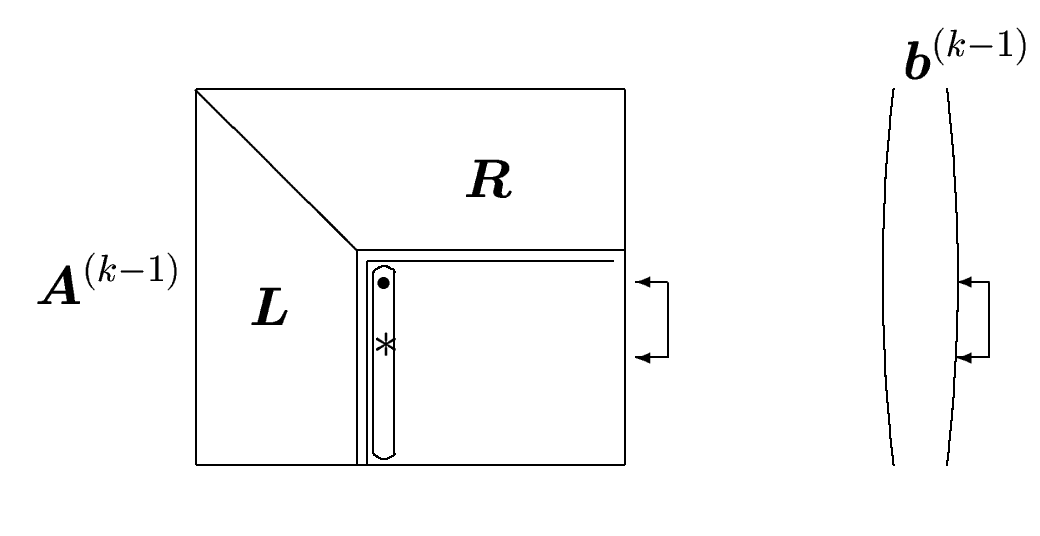
\includegraphics[width=0.5\linewidth]{images/Gausspivot.png}
\end{image}

\begin{enumerate}[1.]
\item Bestimme das Pivotelement $a_{pk}^{(k-1)}$ 
  als betragsmäßig größtes der \enquote{Rest-Spalte}, d.h.
  \begin{gather*}
    |a_{pk}^{(k-1)}|\geq |a_{jk}^{(k-1)}| \qquad  \text{ für } j=k,\ldots , n
  \end{gather*}
\item Vertausche in $A^{(k-1)}$ die $k$-te mit der $p$-ten Zeile
\item Führe einen Gauß-Eliminationsschritt aus.
\end{enumerate}

\begin{Beme}~
  \begin{enumerate}[a)]
  \item Hiermit gilt $|l_{jk}| \ll 1$.
  \item Anstelle von Spaltenpivotisierung kann eine \textbf{Zeilenpivotisierung}\index{Pivotisierung!Zeilen-}
    durchgeführt werden.
    Welche günstiger (in cpu-time) ist, hängt von der Rechnerarchitektur und
    der damit zusammenhängenden Umsetzung des Gauß-Algorithmus ab.\\
    (Beispielsweise greifen Vektorrechner entweder auf die gesamte Spalte
    oder auf die gesamte Zeile einer Matrix zu und bevorzugen dementsprechend
    Operationen spalten- bzw. zeilenweise.)
  \item Der Aufwand enthält (bis auf $|\cdot |$) keine Rechenoperationen (flops),
    aber $\mathcal{O}(n^2)$ Vergleiche und Vertauschungen.
  \item Eine \textbf{vollständige Pivotsuche}\index{Pivotisierung!vollständige} sucht das betragsmäßig größte Element der gesamten Restmatrix und benötigt $\mathcal{O}(n^3) $ Vergleiche
    (sie wird so gut wie nie angewendet).
  \end{enumerate}
\end{Beme}

Damit die LR-Zerlegung unabhängig von der rechten Seite erstellt werden kann, müssen die Permutationen gespeichert werden.
Hierfür verwendet man  einen sog. \textbf{Permutationsvektor} $\Pi$, wobei
\begin{gather*}
  \Pi^{(k-1)}(r) = s
\end{gather*}
bedeutet, dass nach dem $(k-1)$-ten Eliminationsschritt in der $r$-ten Zeile
von $A^{(k-1)}$ die $s$-te bearbeitete Zeile von $A$ steht, also
\begin{align*}
  \Pi^{(k)}(k) &= \Pi^{(k-1)}(p) \\
  \Pi^{(k)}(p) &= \Pi^{(k-1)}(k)  \quad \text{und entsprechend} \\
  \scriptsize \Pi^{(k)} (i) &= \Pi^{(k)} (i) \quad \text{ für }  i\neq k,p 
\end{align*}
Für die \textbf{Permutationsmatrix}\index{Permutationsmatrix}
$P_{\Pi}$ gilt: 
\begin{align*}
  P_{\Pi}&\coloneqq (e_{\Pi(1)}, \ldots , e_{\Pi(n)}) 
  & e_j\coloneqq 
    {\scriptsize\begin{pmatrix}0\\\vdots\\0\\1\\0\\\vdots\\0\end{pmatrix}
  \begin{array}{l}\\\\\shortleftarrow \text{$j$-te Stelle}\\\\\\\end{array}}\\
  PA&= LR \\
  P^{-1} &= P^T
           \det P_{\Pi} = \Sign(\Pi) 
           % \\
           % &=  \begin{cases}
           %   +1&  \text{falls }\Pi \text{ von gerader}\\
           %   -1 &  \text{falls } \Pi \text{ von ungerader}
           % \end{cases} \text{ Anzahl an Transpositionen erzeugt wird}
\end{align*}


\subsectione{Algorithmus: Gauß-Elimination mit Spaltenpivotisierung}\label{2.2.3}
Der zugehörige Algorithmus zur Spaltenpivotisierung ist: \\

\begin{pseudocode}{0.9\linewidth}
  $\pi(1 : n) = [1 : n] $  \\
  \textbf{for} $k = 1, \dots, n-1$ \\
  ~|	  \> bestimme Pivotzeile $p$, so dass\\
  ~|	  \>\>	$|a_{pk} | = \max\{|a_{jk} | , j = k, . . . , n\}$ \\
  ~|	  \> $\pi(k) \leftrightarrows\footnotemark \pi(p)$ \\
  ~|	  \> $A(k, 1 : n) \leftrightarrows A(p, 1 : n)$ \\
  ~|	  \> \textbf{if} $a_{kk} \neq 0$ \\
  ~|	  	   \>~|\> $zeile = [k + 1 : n]$ \\
  ~|	  	   \>~|\> $A(zeile, k) = A(zeile, k)/a_{kk}$ \\
  ~|	  	   \>~|\> $A(zeile, zeile) = A(zeile, zeile) - A(zeile, k)A(k, zeile)$\\
  ~|	  \> \textbf{else} \\
  ~|	  	   \>~|\> \enquote{$A$ ist singulär}\\
  ~|	  \> \textbf{end}\\
  \textbf{end}
\end{pseudocode}	\footnotetext{$\leftrightarrows$ bedeutet \enquote{vertausche mit}}
\\

\begin{Satze}[Dreieckszerlegung mit Permutationsmatrix] \label{2.2.4} 
  Für jede invertierbare Matrix $A$ existiert eine Permutationsmatrix $P$,
  so dass eine Dreieckszerlegung
  \begin{gather*}
    PA = LR
  \end{gather*}
  existiert.
  $P$ kann so gewählt werden, dass alle Elemente von $L$ betragsmäßig kleiner oder gleich
  1 sind, d.h.
  \begin{gather*}
    |l_{ij}| \leq 1\quad \forall i, j
  \end{gather*}
\end{Satze}


\begin{proof}
  Da $\det A \neq 0$ ist, existiert eine Transposition $\tau_1$, s.d. 
  \begin{gather*}a_{11}^{(1)}= a_{\tau_1, 1} \neq 0 \end{gather*}
  und
  \begin{gather*}
    | a_{\tau_1, 1} | \geq |a_{i1}| 
    \quad \forall i=1, \cdots, n \, . 
  \end{gather*}
  Wir erhalten damit
  \begin{gather*}
    L_1P_{\tau_1} \cdot A = A^{(1)} = \begin{pmatrix}
      a_{11}^{(1)} && \cdots ~&  ~\\
      0 \\
      \vdots && B^{(1)} \\
      0
    \end{pmatrix}
  \end{gather*}
  und alle Elemente von $L_1 $ sind betragsmäßig kleiner oder gleich 1 sowie
  $\det L_1 = 1 $. \\
  Daraus folgt
  \begin{align*}
    \det B^{(1)} & = \frac{1}{\underbrace{a_{11}^{(1)}}_{\neq 0}} \cdot \det A^{(1)} \\
                 & = \frac{1}{a_{\tau_1, 1}^{(1)}}\cdot \det (L_1) \cdot \det (A) \\
                 & \neq 0 \, .
  \end{align*}
  Also ist $B^{(1)}$ invertierbar. \\
  
  Induktiv erhalten wir dann
  \begin{gather*}
    R = A^{(n-1)} = L_{n-1}P_{\tau_{n-1}} \cdot \dotsc \cdot L_1 P_{\tau_1} \cdot A
  \end{gather*}\\
  
  % ------------------------------------------------------

  Da $\tau_i$ nur zwei Zahlen $\geq i $ vertauscht, ist
  \marginpar{15.10.2014}
  \begin{align*}\index{Vorwärtselimination}
    \Pi_i  &\coloneqq \tau_{n-1} \circ \ldots \circ \tau_i \quad\text{ für } i=1,\ldots (n-1) 
  \end{align*}
  eine Permutation der Zahlen $\{i,\dots, n\}$, d.h. insbesondere gilt:
  \begin{alignat*}{2}
    \Pi_i(j)&=j  & \quad &\text{ für } j=1,\dots,(i-1) \\
    \Pi_i(j)&\in \{i, \dots, n\} & &\text{~für~}j=i,\dots, n\,. 
  \end{alignat*}
  \begin{align*}
    P _{\Pi_{i+1}}  &= (e_1, \dotsc e_i, e_{\Pi_{i+1}(i+1)}, \dotsc, e_{\Pi_{i+1}(n)}) 
                      = \begin{pmatrix}
                        I_i & 0 \\
                        0 & P_{\sigma}
                      \end{pmatrix}
  \end{align*}
  Damit folgt:
  \begin{align*}
    P_{\Pi_{i+1}}\cdot L_i\cdot P_{\Pi_{i+1}}^{-1}
    &= P_{\Pi_{i+1}} \cdot 
      \left(\begin{array}{ccc|ccc}
              & I_i & && 0 & \\
              \cline{1-6}
              & & -l_{i+1, i} & & & \\
              &  0 &  \vdots  & & I_{n-i} &\\
              &    & -l_{n, i} & &  & 
            \end{array}\right)
                                      \cdot\begin{pmatrix}
                                        I_i & 0 \\
                                        0 & P_{\sigma}^{-1}
                                      \end{pmatrix}\\
    &= \begin{pmatrix}
      I_i & 0 \\
      0 & P_{\sigma}
    \end{pmatrix}
          \cdot   \ldots  \cdot
          \left(\begin{array}{ccc|ccc}
                  & I_i & && 0 & \\
                  \cline{1-6}
                  \cdot & & -l_{i+1, i} & & & \\
                  &  0 &  \vdots      & & P_{\sigma}^{-1} &\\
                  &     & -l_{n, i} & &  & 
                \end{array}\right) \\
    &= \left(\begin{array}{ccc|ccc}
               & I_i & && 0 & \\
               \cline{1-6}
               &     & -l_{\Pi_{i+1}(i+1), i} & & & \\
               &  0 &  \vdots      & & I_{n-i} &\\
               &     & -l_{\Pi_{i+1}(n), i} & &  & 
             \end{array}\right) \\
    &= I - (P_{\Pi_{i+1}} l_i)e_i^T\\
    &\eqqcolon \widehat{L}_i
  \end{align*}
  und
  \begin{align*}		R =&\, L_{n-1}\\
                           &\cdot (P_{\tau_{n-1}}L_{n-2}P_{\tau_{n-1}}^{-1})\\
                           &				\cdot (P_{\tau_{n-1}}P_{\tau_{n-2}}L_{n-2}P_{\tau_{n-2}}^{-1}P_{\tau_{n-1}}^{-1})\\
                           &\; \vdots \\
                           &		 \cdot (P_{\tau_{n-1}}\dotsm P_{\tau_{1}}L_{1}P_{\tau_{1}}\dotsm P_{\tau_{n-1}}) \cdot A\\
    =&\,L_{n-1}\widehat{L}_{n-2}\dotsm\widehat{L}_1P_{\Pi_{1}}\cdot A
  \end{align*}
  Nach Lemma \autoref{2.1.12} gilt daher, es existiert eine Permutation $\Pi_{1}$ mit
  \begin{gather*}
    P_{\Pi_1}\cdot A = LR ,
  \end{gather*}
  wobei $R$ obere Dreiecksgestalt hat und
  \begin{align*}
    L  &=  \begin{pmatrix}
      1 && & 0\\
      l_{\Pi_2(2),1} & \ddots & \\
      \vdots &            \ddots &  1\\
      l_{\Pi_n(n),1}& \dotsm &  l_{\Pi_n(n),n-1} & 1 
    \end{pmatrix} 
                     & \text{mit } |l_{ij}| \leq 1 
  \end{align*}
  gilt.
\end{proof}

\subsectione{Lösen eines Gleichungssystems $Ax=b$} 
Das Lösen eines linearen Gleichungssystems der Form $Ax=b$ wird mittels
Elimination durch folgende drei Schritte durchgeführt:
\begin{enumerate}[1)]
\item Zerlege $A$ durch $PA=LR$
\item Löse durch Vorwärtssubstitution $Lz=Pb$
\item Löse durch Rückwärtssubstitution $Rx=z$
\end{enumerate}

% \subsectione{Bemerkungen}
\begin{Beme}~
  \begin{enumerate}[a)]
  \item $P_\Pi A=LR$ kann zur Berechnung von $\det(A)$ genutzt werden
    (allgemeine Formel: $\det(A)=\Sign(\Pi)\cdot r_{11}\cdot \ldots \cdot r_{nn}$).
  \item Algorithmus \ref{2.2.3}  testet, ob die Matrix singulär ist,
    bis auf den Fall $r_{nn}=a_{nn}^{(n-1)}=0$.
  \item $\det(A)=0$ sollte nicht als (numerischer) Nachweis für die
    Singularität von $A$ genutzt werden.\\
    Z.B. ist $10^{-8}I$ regulär, aber $\det(10^{-8}I) = 10^{-8n}$ ist fast 0
    für große $n$, also ist $A$ numerisch singulär.
  \end{enumerate}
\end{Beme}

% \subsectione{Beispiel zur Pivotisierung}
\begin{Bspe}
  Wir betrachten die Pivotisierung mit betragsmäßig größtem Spaltenelement
  und Rundungsfehlern zu
  \begin{gather*}
    A=\begin{pmatrix}
      10^{-4} & 1 \\ 1 & 1
    \end{pmatrix}, ~
    b= \begin{pmatrix*}
      1 \\ 2
    \end{pmatrix*}\, .
  \end{gather*}
  Die der Gauß-Elimination mit Rundung auf 3 Dezimalstellen ergibt
  $l_{21}=10^4$, denn kleines Pivotelement bedeutet großer Multiplikator. \\
  \begin{align*}
    r_{22}&=a_{22}-l_{21}a_{12} = 1-10^4\cdot 1 = -999 \approx -10^4 \eqqcolon \widetilde{r}_{22}\\
    b_2^{(1)} & = b_2-l_{21}b_1 = 2-10^4 = -9998 \approx -10^4 \eqqcolon \widetilde{b}_2^{(1)} 
  \end{align*}
  Die Rückwärtssubstitution ergibt
  \begin{align*}
    x_2 &= \frac{-b_2^{(1)}}{r_{22}} = \frac{9998}{9999} \approx 1\\
    \widetilde{x}_	2 &= \frac{\widetilde{b}_2}{\widetilde{r}_{22}} = \frac{-10^4}{-10^4} = 1 \\\\
    x_1 &= \frac{1}{r_{11}}(b_1-r_{12}x_2)= 10^4 (1-1x_2) = \frac{10^4}{9999}\approx 1\\
    \widetilde{	x}_1 &= \frac{1}{\widetilde{r}_{11}}(1-1\widetilde{x}_2)= 10^4 (1-1\cdot 1) = 0 
  \end{align*}
  Dies führt zu einem starken Fehler.\\
  
  Mit Spaltenpivotisierung ist $l_{21}=10^{-4}<1$ und 
  $\widetilde{r}_{22}=1$, $b_2^{(2)} = 1$, $\widetilde{x}_2=1$, $\widetilde{x}_1=1$.\\
  Diese Werte führen auch bei Rundungsfehlern zu besseren Ergebnissen.
\end{Bspe}

% -----------------------------------------------------------------------
%%% Local Variables:
%%% mode: latex
%%% TeX-master: "../numerik_script"
%%% End:
